\subsection{M.PC.SV - Schedule Variance e M.PC.CV - Cost Variance}

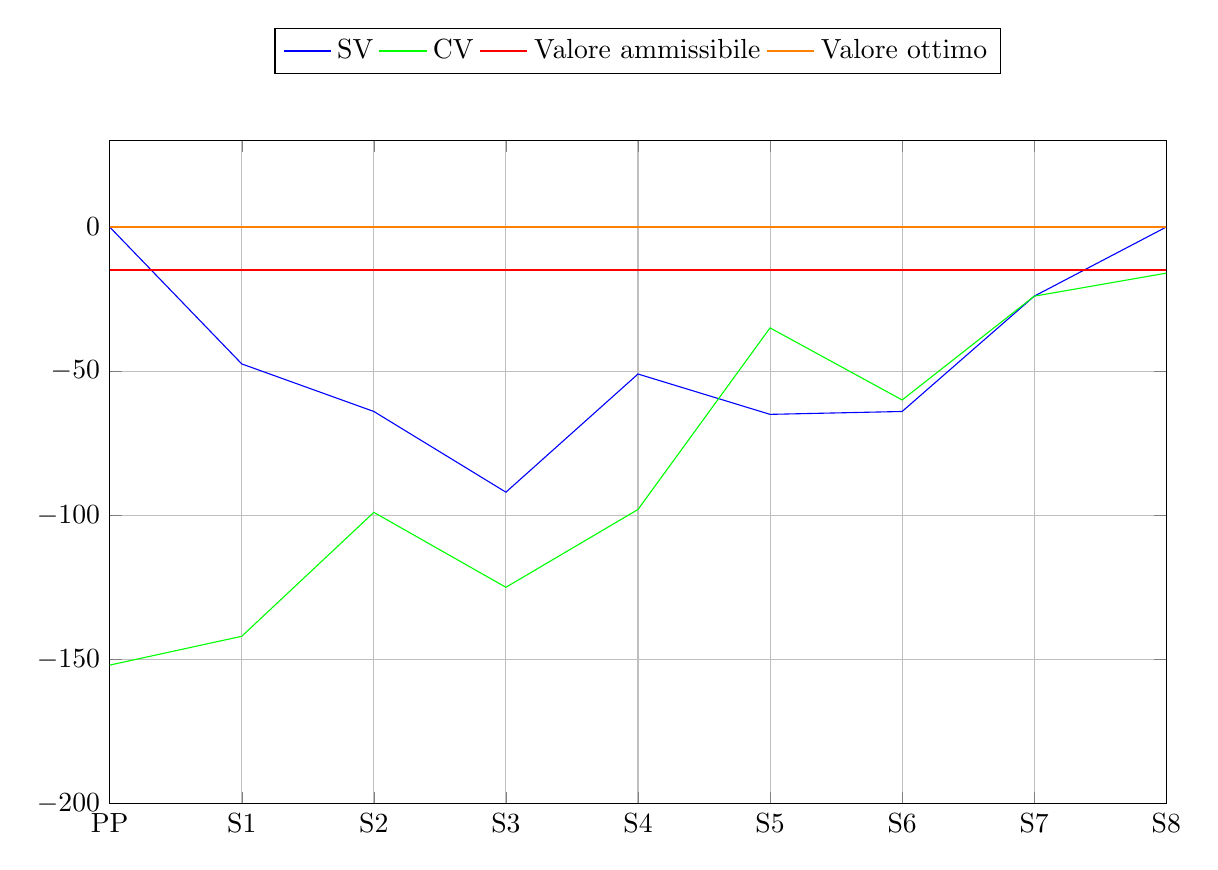
\begin{tikzpicture}
    \begin{axis}[
        width=15cm, height=10cm,
        ymin=-200, ymax=30,
        xmin=0, xmax=8,
        xtick={0, 1, 2, 3, 4, 5, 6, 7, 8},
        xticklabels={ PP, S1, S2, S3, S4, S5, S6, S7, S8},
        xlabel={},
        ylabel={},
        grid=major,
        scaled ticks=false,
        legend style={at={(0.5,1.1)}, anchor=south, legend columns=-1},
    ]
    \addplot[color=blue] coordinates {(0, 0) (1, -47.5) (2, -64) (3, -92) (4, -51) (5, -65) (6, -64) (7, -24) (8, 0)};
    \addlegendentry{SV}
    \addplot[color=green] coordinates {(0, -152) (1, -142) (2, -99) (3, -125) (4, -98) (5, -35) (6, -60) (7, -24) (8, -16)};
    \addlegendentry{CV}
    \addplot[red, thick] coordinates {(0, -15) (8, -15)};
    \addlegendentry{Valore ammissibile}
    \addplot[orange, thick] coordinates {(0, 0) (8, 0)};
    \addlegendentry{Valore ottimo}
    \end{axis}
\end{tikzpicture}
\subsubsection{RTB}
La \glossario{Schedule Variance} (SV) presenta valori negativi e significativamente inferiori al valore ammissibile. 
Questo fenomeno è principalmente dovuto a una pianificazione troppo ottimistica e inaccurata delle attività. 
Come evidenziato dal grafico, l'\glossario{Earned Value} (EV) per ogni sprint è stato notevolmente più basso rispetto al \glossario{Planned Value} (PV), causando un valore di SV costantemente negativo e lontano dagli obiettivi prefissati. 
Durante lo Sprint 5 è stata effettuata una pianificazione per completare tutte le attività necessarie al \glossario{Proof of Concept}. 
Tuttavia, queste attività non sono state completate nei tempi previsti, determinando un ulteriore calo di SV.
La \glossario{Cost Variance} (CV), pur rimanendo negativa, mostra un miglioramento progressivo. Questo accade perché le ore di lavoro dedicate ad attività non completate durante uno sprint comportano un incremento del costo reale (\glossario{Actual Cost} - AC) senza un corrispondente incremento di EV.
Tuttavia, quando queste attività vengono completate negli sprint successivi entro il tempo preventivato, la CV migliora. 
Questo si verifica perché l'EV aumenta notevolmente, mentre l'AC cresce solo marginalmente per il completamento delle attività.